\documentclass[a4paper]{article}
% Leave uncommented if the LaTeX file is uploaded to arXiv.org
\pdfoutput=1
\pdfminorversion=7

% Packages
\usepackage{arxiv}
\usepackage[colorlinks=true,linkcolor=blue,citecolor=blue]{hyperref}
\usepackage[numbers]{natbib}
\usepackage{authblk}
\usepackage{graphicx}
\usepackage{amsmath}
\usepackage{amssymb}
\usepackage{epstopdf}
\usepackage{comment}
\usepackage{xcolor}
\usepackage{float}
\usepackage{doi}

% Useful macros for equations and units in HEP
\newcommand*{\TeV}{\text{ TeV}}
\newcommand*{\GeV}{\text{ GeV}}
\newcommand*{\MeV}{\text{ MeV}}
\newcommand*{\keV}{\text{ keV}}
\newcommand*{\eV}{\text{ eV}}
\newcommand*{\meV}{\text{ meV}}
\newcommand*{\bb}{\boldsymbol}
\newcommand*{\beqn}{\begin{equation}}
\newcommand*{\eeqn}{\end{equation}}
\newcommand{\req}[1]{Eq.\,(\ref{#1})}
\newcommand{\rf}[1]{Fig.~{\ref{#1}}}
\newcommand{\rsec}[1]{Sect.\,{\ref{#1}}}

% Useful macros for annotation
\newcommand*{\xred}{\color{red}}
\newcommand*{\xblue}{\color{blue}}
\newcommand*{\xgreen}{\color{green}}

\title{\boldmath Magnetic Properties of Finite Temperature Primordial Electron-Positron Plasma}

% Author Orcid ID: Define per author
\newcommand{\orcA}{0000-0001-8217-1484}
\newcommand{\orcB}{0000-0001-5038-8427}
\newcommand{\orcC}{0000-0001-5474-2649}

\author{Andrew Steinmetz\orc{\orcC}\thanks{Correspondence: \texttt{ajsteinmetz@arizona.edu}}, Cheng Tao Yang\orc{\orcB}, and Johann Rafelski\orc{\orcA}\\ Department of Physics, The University of Arizona, Tucson, AZ 85721, USA}

\begin{document}

\maketitle

\begin{abstract}
    We explore the possibility of magnetization within the primordial electron-positron plasma in the temperature range $2000\keV>T>20\keV$ where the $e^{+}e^{-}$ pair density was up to $10^{9}$ greater than the baryon density. We suggest that primordial magnetization within the plasma is driven by spin paramagnetism. At these high densities, strong dampening by internal scattering needs to be included in any study of magneto-hydrodynamic flow. The rapid disappearance of $e^{+}e^{-}$ at temperatures $T<511\keV$ occured much faster than the corresponding drop in temperature.
\end{abstract}

\keywords{early universe cosmology \and magnetization \and electron-positron plasma \and intergalactic magnetic fields}

%%%%%%%%%%%%%%%%%%%%%%%%%%%%%%%%%%%%%%%
\section{Introduction}
\label{sec:introduction}
\noindent Macroscopic domains of magnetic fields have been found: around compact objects (stars, planets, etc...), between stars, within galaxies, between galaxies in clusters, and surprisingly in the deep extra-galactic void spaces where little matter exists. Therefore we search for a common mechanism that could produce the magnetic diversity we see in today's contemporary universe. Unlike electric fields which cannot be supported at large scales due to the charge neutrality of the universe, cosmic magnetic fields are easily generated~\cite{kronberg1994extragalactic} by a variety of physicals phenomenon which are difficult to screen. In the early universe above temperature $T>20\keV$ there was an gargantuan density of electron-positron pairs which rapidly vanished as the universe cooled~\cite{rafelski2023short}. We explore the possibility that this phenomenon was responsible for generating primordial magnetic fields (PMF) in the universe. We note that above temperature $T\gtrsim85\keV$, the $e^{+}e^{-}$ primordial plasma density exceeded that of the Sun's core density $n_{e}\simeq6\times10^{26}{\rm\ cm}^{-3}$~\cite{bahcall2001solar}. We analyze the magnetized relativistic fermion partition function focusing on the spin contribution to magnetization showing that magnetization is nonzero even for a nearly symmetric particle-antiparticle gas. At higher electron-positron $e^{+}e^{-}$ pair densities, spin paramagnetism is dominant over the Landau orbital diamagnetism of the gas.

If the early universe was highly magnetized, the rapid $10^{9}$ drop in $e^{+}e^{-}$ density relative to the baryon density in the temperature range $2000\keV>T>20\keV$ likely had a large effect on the overall magnetization of the universe. This combination of strong magnetic fields, high matter-antimatter density, and relatively high temperatures (far higher than the Sun's core temperature~\cite{bahcall2001solar} of $T_{\odot}=1.37\keV$) make this era unique in cosmology and astrophysics. We operate under the assumption that the observed inter-galactic magnetic fields (IGMF) are primordial in nature and are present, if not created fully or in part, during the electron-positron epoch of the early universe. The conventional elaboration of the origins for IGMFs are detailed in~\cite{gaensler2004origin,durrer2013cosmological,batista2021gammaray}.

These intergalactic fields present a challenge both experimentally and theoretically in that they are (a) difficult to measure and (b) difficult to explain using known physics. The bounds for IGMF at a coherent length scale of $1{\rm\ Mpc}$ are today~\cite{neronov2010evidence,taylor2011extragalactic,pshirkov2015new,vernstrom2021discovery}
\begin{align}
    \label{igmf}
    10^{-8}{\rm\ G}>\mathcal{B}_{\rm IGFM}>10^{-16}{\rm\ G}\,.
\end{align}

Faraday rotation from distant radio active galaxy nuclei (AGN)~\cite{pomakov2022redshift} suggest that neither dynamo nor astrophysical processes would sufficiently account for the presence of IGMF in the universe today if the IGMF strength was around the upper bound of ${\cal B}_{\rm IGMF}\simeq30-60{\rm\ nG}$ as found in~\cite{vernstrom2021discovery}. Such strong IGMFs would then require that at least some portion of the IGMF arise from primordial sources that predate the formation of stars and galaxies, or the cosmic microwave background (CMB). It was shown by Jedamzik and Pogosian~\cite{jedamzik2020relieving} that the presence of ${\cal B}_{\rm PMF}\simeq0.1{\rm\ nG}$ could be sufficient to explain the Hubble tension. Such pre-recombination PMFs would lead to early universe baryon inhomogeneities which in turn would produce anisotropies in the CMB~\cite{jedamzik2013smallscale}. PMF strengths of around a tenth of a nanoGauss is also near the more stringent upper bound for PMFs found in~\cite{pshirkov2015new,jedamzik2019stringent}. Conversely, measurements of synchrotron radiation from \lq\lq blazar\rq\rq\ AGN whose jets are pointed towards the Earth provide the lower bound~\cite{neronov2010evidence,taylor2011extragalactic} on IGMFs seen in \req{igmf}. Due to cosmological redshift, and the conservation of magnetic flux through a comoving surface, PMFs would have extraordinary field strengths during the various primordial plasmas of the early universe subject to whatever temperature they were initially generated in.

%%%%%%%%%%%%%%%%%%%%%%%%%%%%%%%%%%%%%%%
\section{Electron-positron abundance}
\label{sec:abundance}
%%%%%%%%%%%%%%%%%%%%%%%%%%%%%%%%%%%%%%%
\begin{figure}[ht]
    \centering
    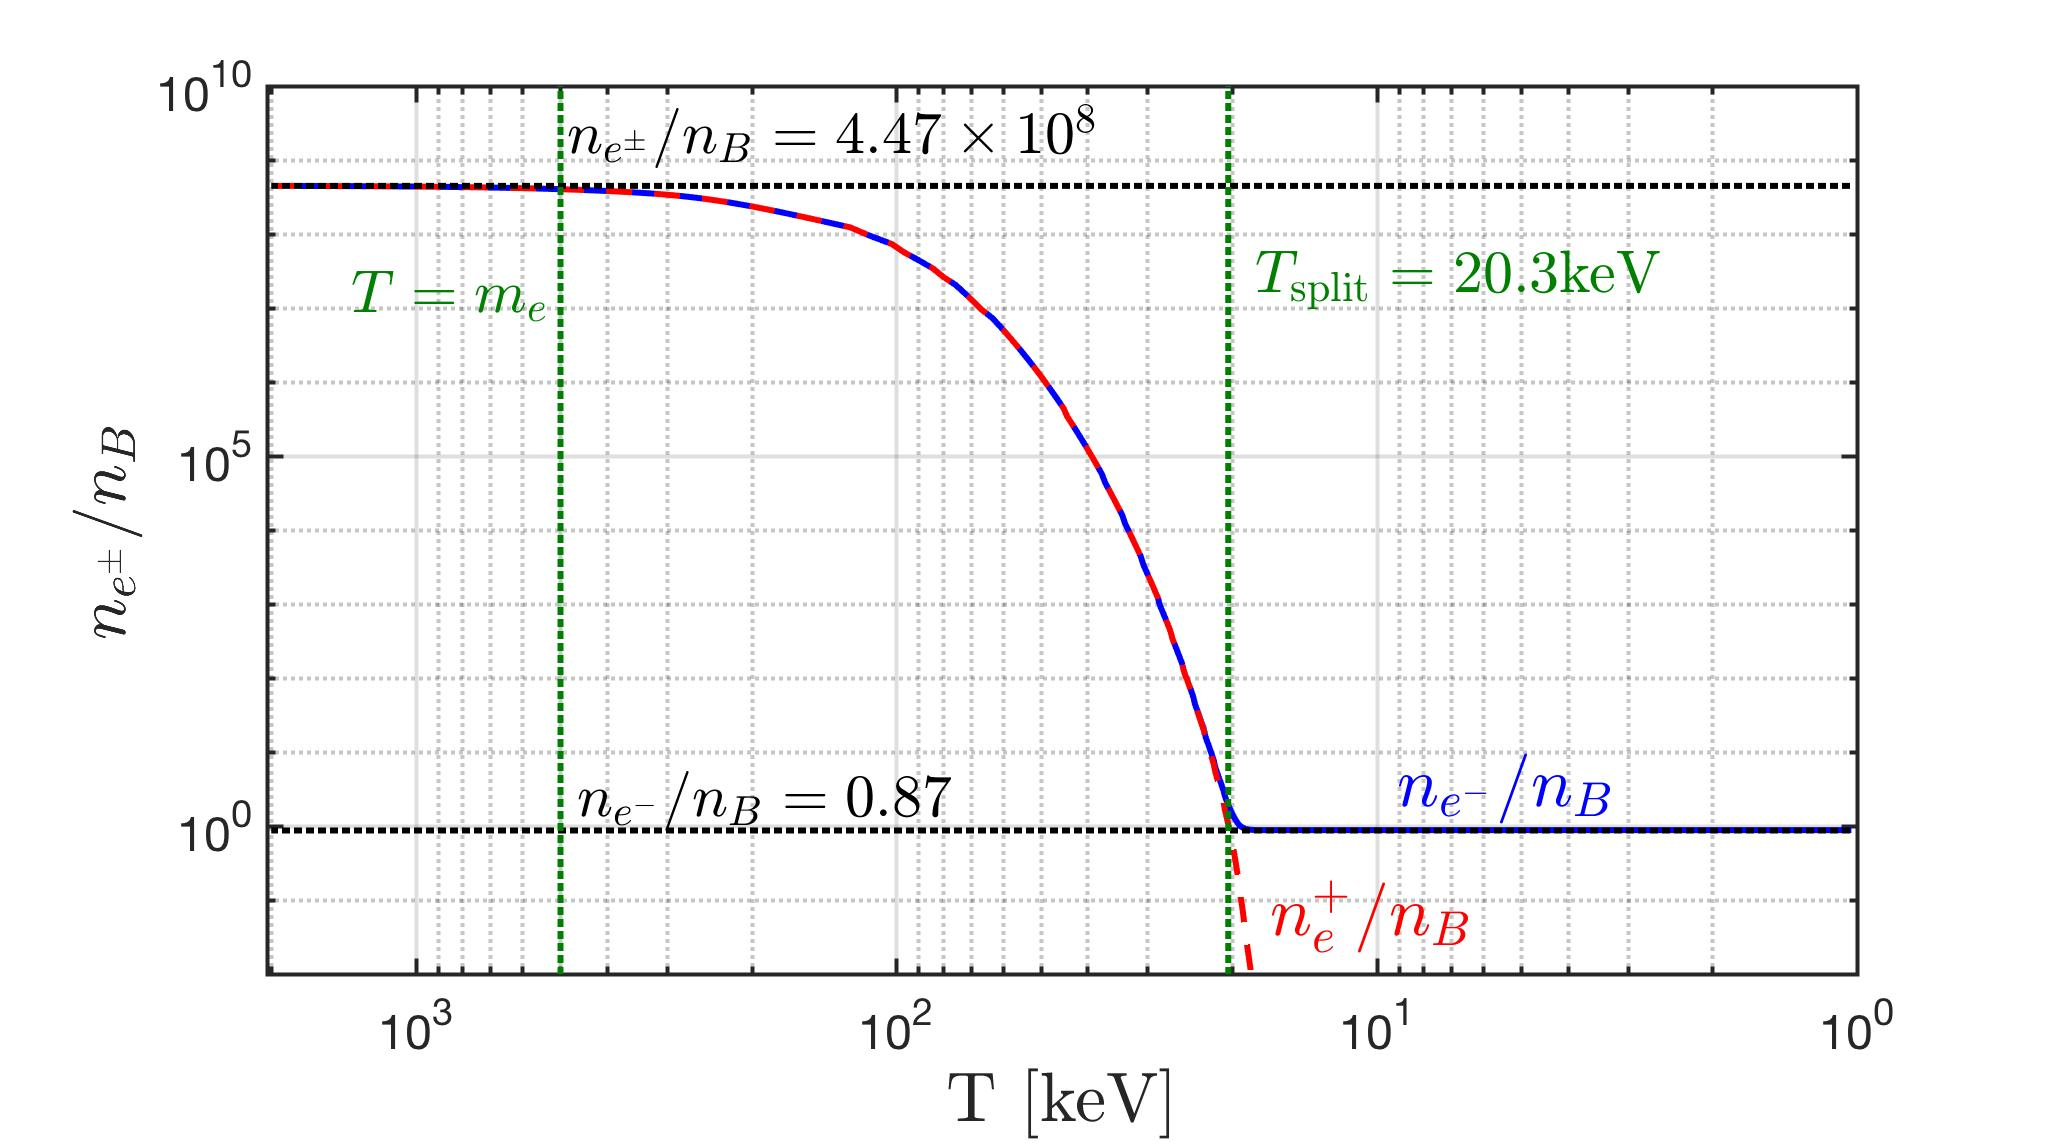
\includegraphics[width=\textwidth]{EEPlasmaDensityRatio.jpg}
    \caption{The light charged lepton-to-baryon ratio $n_{e^{\pm}}/n_{B}$ is plotted as a function of temperature. The electron-to-baryon ratio $n_{e^{-}}/n_{B}$ is shown as the solid blue line while the positron-to-baryon ratio $n_{e^{+}}/n_{B}$ is printed as the dashed red line. The two vertical dashed green lines denote temperatures $T=m_{e}\simeq511\keV$ and $T=20.3\keV$. The two horizontal black dashed lines denote the pre-annihilation constant of $n_{e^{\pm}}/n_{B}=4.47\times10^{8}$ and post-annihilation constant of $n_{e^{-}}/n_{B}=0.87$.}
    \label{densityratio} 
\end{figure}
%%%%%%%%%%%%%%%%%%%%%%%%%%%%%%%%%%%%%%%

\noindent In \rf{densityratio} we present the electron-positron number density ratio relative to the baryon number density in the temperature range $2000\keV>T>20\keV$ which bounded the $e^{+}e^{-}$ epoch of the early universe. After neutrino freeze-out~\cite{birrell2014relic}, around $T=2\MeV$, the comoving density of $e^{+}e^{-}$ remained constant fixed to a value of 
\begin{align}
    \label{comovingdensity}
    \frac{n_{e^{+}}+n_{e^{-}}}{n_{B}}\simeq0.9\times10^{9}\,,
\end{align}
or almost 1 billion times more abundant than the baryons. Constancy of this ratio for temperature above $T\gtrsim500\keV$ originates from the conserved entropy-per-baryon ratio~\cite{fromerth2012quarkgluon}. This indicates that the entropy content in the light charged leptons was also constant and conserved during this period. As the universe cooled below temperature $T<m_{e}$ (the electron mass), the electron and positron comoving density depleted (falling nine orders of magnitude) as the annihilation process outpaced the photon fusion pair production process via
\begin{align}
    \label{fusion}
    e^{+}+e^{-}\leftrightarrow\gamma+\gamma\,.
\end{align}
At $T=20.3\keV$, the charged lepton asymmetry (mirrored by the baryon asymmetry) became evident as the few remaining excess electrons could no longer annihilate as the positrons vanished entirely. This process took no longer than an afternoon lunch break. Because of charge neutrality, the post-annihilation comoving ratio $n_{e^{-}}/n_{B}=0.87$~\cite{rafelski2023short} is slightly offset from unity by the presence of $\alpha$ particles and the other neutron containing light elements produced during Big Bang nucleosynthesis (BBN).

%%%%%%%%%%%%%%%%%%%%%%%%%%%%%%%%%%%%%%%
\section{Primordial magnetic fields}
\label{sec:primordial}
\noindent As the universe undergoes isotropic expansion, the temperature decreases as 
\begin{align}
    \label{tscale}
    T(t)=T_{0}\frac{a_{0}}{a(t)}\rightarrow T(z)=T_{0}(1+z)\,,
\end{align}
where $a(t)$ is the scale factor defined by the FLRW metric~\cite{weinberg1972gravitation} and $z$ is the redshift. The comoving temperature $T_{0}$ is given by the present day temperature of the CMB and the contemporary scale factor $a_{0}=1$ is usually set to unity. Within a homogeneous magnetic domain, the magnetic field varies~\cite{durrer2013cosmological} over cosmic expansion as
\begin{align}
    \label{bscale}
    {\cal B}(t)={\cal B}_{0}\frac{a_{0}^{2}}{a^{2}(t)}\rightarrow{\cal B}(z)={\cal B}_{0}\left(1+z\right)^{2}\,,
\end{align}
where ${\cal B}_{0}$ is the comoving value of the magnetic field defined by the contemporary value of the magnetic field today given in \req{igmf}. Non-primordial magnetic fields which are generated through other mechanisms (such as dynamo or astrophysical sources) will have expressions which differ~\cite{pomakov2022redshift}. The presence of matter and late universe structure formation also serve to contaminate the primordial field evolution in \req{bscale}, therefore it is only in deep intergalactic space where primordial fields would remain preserved over cosmic time.

From \req{tscale} and \req{bscale}, we see there is a natural ratio which is conserved over cosmic expansion. For particles (such as $e^{+}e^{-})$ with charge magnitude $q=|e|$ in a homogeneous primordial magnetic field, we can define a dimensionless cosmic magnetic energy scale in natural units ($c=\hbar=k_{B}=1$) as
\begin{align}
    \label{tbscale}
    b_{0}\equiv\frac{q{\cal B}(t)\hbar c^{2}}{k_{B}^{2}T^{2}(t)}\rightarrow\frac{q{\cal B}(t)}{T^{2}(t)}=\frac{q{\cal B}_{0}}{T_{0}^{2}}={\rm\ const.}\qquad10^{-3}>b_{0}>10^{-11}\,,
\end{align}
which can be completely prescribed by comoving values. We compute the bounds for this cosmic magnetic scale by using the present day observations given by \req{igmf} and the CMB temperature $T_{0}=2.7{\rm\ K}$~\cite{aghanim2018planck}.

We take inspiration from Ch. 9 of Melrose's treatise on magnetized plasmas~\cite{melrose2008quantum}. Our focus however will be on the bulk properties of thermalized plasmas in (near) equilibrium. In considering $e^{+}e^{-}$ plasma, we introduce the microscopic energy of the charged $q$ relativistic fermion within a homogeneous ($z$-direction) magnetic field~\cite{steinmetz2018magnetic}. The energy eigenvalue is given by
\begin{align}
    \label{kgp}
    E^{\pm}_{n}(p_{z},{\cal B})=\sqrt{m_{e}^{2}+p_{z}^{2}+q{\cal B}\left(2n+1\mp\frac{g}{2}\right)}\,,\qquad n\in0,1,2,\ldots
\end{align}
where $p_{z}$ is the momentum parallel to the field axis and $n$ is the Landau orbital quantum number. The subscript $\pm$ refers to the spin polarization along the field axis: parallel $(+)$ or anti-parallel $(-)$. The parameter $g$ is the gyro-magnetic ($g$-factor) of the particle. We rearrange \req{kgp} by pulling the spin dependency and the ground state Landau orbital into the mass writing
\begin{align}
    \label{effmass}
    E^{\pm}_{n}={\tilde m}_{\pm}\sqrt{1+\frac{p_{z}^{2}}{{\tilde m}_{\pm}^{2}}+\frac{2q{\cal B}n}{{\tilde m}_{\pm}^{2}}}\,,\qquad {\tilde m}_{\pm}^{2}=m_{e}^{2}+q{\cal B}\left(1\mp\frac{g}{2}\right)\,,
\end{align}
where we introduced the effective polarized mass ${\tilde m}_{\pm}$ which is distinct for each spin alignment and is a function of magnetic field strength ${\cal B}$. The effective polarized mass ${\tilde m}_{\pm}$ allows us to describe the $e^{+}e^{-}$ plasma with the spin effects almost wholly separated from the Landau characteristics of the gas when considering plasma thermodynamic properties.

%%%%%%%%%%%%%%%%%%%%%%%%%%%%%%%%%%%%%%%
\section{Magnetized fugacity}
\label{sec:fugacity}
\noindent The magnetized relativistic fermion partition function is given, in a generalized form, by
\begin{align}
    \label{partition}
    \ln{\cal Z}_{e^{+}e^{-}}=\frac{2q{\cal B}V}{(2\pi)^{2}}\sum_{\sigma}^{\pm}\sum_{s}^{\pm}\sum_{n=0}^{\infty}\int_{0}^{\infty}\left[\ln\left(1+\lambda_{\sigma}\xi_{s}e^{-E_{n}^{s}/T}\right)\right]\,,\qquad\Upsilon_{\sigma}^{s}=\lambda_{\sigma}\xi_{s}=\exp{\frac{\mu_{\sigma}+\eta_{s}}{T}}\,,
\end{align}
where $\sigma$ is a sum over electron and positron states and $s$ is a sum over polarizations. We define the generalized fugacity $\Upsilon_{\sigma}^{s}$ as the product of:
\begin{itemize}
    \item[a.] Chemical fugacity $\lambda_{\sigma}=e^{\mu_{\sigma}/T}$
    \item[b.] Spin fugacity $\xi_{s}=e^{\eta_{s}/T}$
\end{itemize}
The chemical fugacity $\lambda_{\sigma}$ is defined in terms of the chemical potential $\mu_{\sigma}=\sigma\mu$ and due to charge conservation~\cite{elze1980relativistic} can be written as 
\begin{align}
    \label{cpotential}
    \mu\equiv\mu_{e^{-}}=-\mu_{e^{+}}\,,\qquad
    \lambda\equiv\lambda_{e^{-}}=\lambda_{e^{+}}^{-1}\,.
\end{align}

While the primordial electron-positron plasma era was overall charge neutral, there was a small asymmetry in the charged leptons from baryon asymmetry~\cite{canetti2012matter} and the presence of protons. Under the condition of charge neutrality, the resulting chemical potential was small~\cite{rafelski2023short} until the universe cooled to a temperature below $T<20\keV$ wherein the positrons vanished from the particle inventory of the universe.

We also introduce a novel spin fugacity $\xi_{s}$ and spin potential $\eta_{s}=s\eta$. While an imbalance in electrons and positrons leads to a nonzero particle chemical potential $\mu\neq0$, an imbalance in spin angular momentum within a region results in a nonzero spin potential $\eta\neq0$. As the universe appears to have zero overall angular momentum, any nonzero spin potential in the electron-positron sector would need to be compensated by either other species in the comoving volume, other sources of angular momentum, or it would indicate the presence of spin magnetized domains not unlike those found in ferromagnetic materials. We propose the spin potential follows analogous expressions as seen in \req{cpotential} obeying
\begin{align}
    \label{spotential}
    \eta\equiv\eta_{-}=-\eta_{+}\,,\qquad
    \xi\equiv\xi_{-}=\xi_{+}^{-1}\,.
\end{align}

We implement the Boltzmann approximation for the limit where $m_e\ll T$ which is approximately true in the temperature range of interest. The Euler-Maclaurin formula~\cite{abramowitz1988handbook} is used to convert the summation over Landau levels into an integration. The resulting partition function can then be written in terms of modified Bessel $K$ functions~\cite{letessier2002hadrons} of the second kind, yielding
\begin{align}
    \label{boltzmann}
    \ln{\cal Z}_{e^{+}e^{-}}\simeq\frac{T^{3}V}{2\pi^{2}}\left[2\cosh{\frac{\mu}{T}}\right]\sum_{s}^{\pm}\xi_{s}\left(x_{s}^{2}K_{2}(x_{s})+\frac{b_{0}}{2}x_{s}K_{1}(x_{s})+\frac{b_{0}^{2}}{12}K_{0}(x_{s})\right)\,,\\
    \label{xfunc}
    2\cosh{\frac{\mu}{T}}=\lambda+\lambda^{-1}\,,\qquad
    x_{\pm}=\frac{{\tilde m}_{\pm}}{T}=\sqrt{\frac{m_{e}^{2}}{T^{2}}+b_{0}\left(1\mp\frac{g}{2}\right)}\,.
\end{align}
The latter two terms in \req{boltzmann} (proportional to $b_{0}K_{1}$ and $b_{0}^{2}K_{0}$) are the uniquely magnetic terms present (containing both paramagnetic and diamagnetic influences) in the partition function while the $K_{2}$ term is present for the relativistic free Fermi gas under the same Boltzmann approximation. As the Bessel $K$ functions are evaluated as functions of $x_{\pm}$ in \req{xfunc}, the \lq\lq free\rq\rq\ part of the partition $K_{2}$ is still subject to spin magnetization effects.

During the $e^{+}e^{-}$ plasma epoch, the density changed dramatically over time changing the chemical potential. Therefore we can utilize the charge neutrality~\cite{rafelski2023short,letessier2002hadrons} of the universe
\begin{align}
    \label{chargeneutrality}
    n_{p}=n_{e^{-}}-n_{e^{+}}=\frac{1}{V}\lambda\frac{\partial}{\partial\lambda}\ln{\cal Z}_{e^{+}e^{-}}
\end{align}
to parameterize the chemical potential $\mu=\mu(T)$ as a function of temperature. The parameter $n_{p}$ is the number density of protons which is known in terms of the baryon-to-photon ratio~\cite{workman2022pdg}. The chemical potential is then
\begin{align}
    \label{chem}
    \sinh{\frac{\mu}{T}}=n_{p}\frac{\pi^{2}}{T^{3}}\left[\sum_{s}^{\pm}\xi_{s}\left(x_{s}^{2}K_{2}(x_{s})+\frac{b_{0}}{2}x_{s}K_{1}(x_{s})+\frac{b_{0}^{2}}{12}K_{0}(x_{s})\right)\right]^{-1}\,.
\end{align}
\req{chem} is fully determined by the right-hand-side expression if the spin fugacity is set to unity $\xi=1$ implying an equal number of polarizations both parallel and anti-parallel to the external field. In general however, an additional constraint is required. We note that such a constraint is likely related to the total angular momentum of the considered volume and does not necessarily imply that spin polarizations must be balanced in a single species when the orbital and spin momentum of all species are taken into account.

%%%%%%%%%%%%%%%%%%%%%%%%%%%%%%%%%%%%%%%
\section{Electron-positron magnetization}
\label{sec:magnetization}
%%%%%%%%%%%%%%%%%%%%%%%%%%%%%%%%%%%%%%%
\begin{figure}[ht]
    \centering
    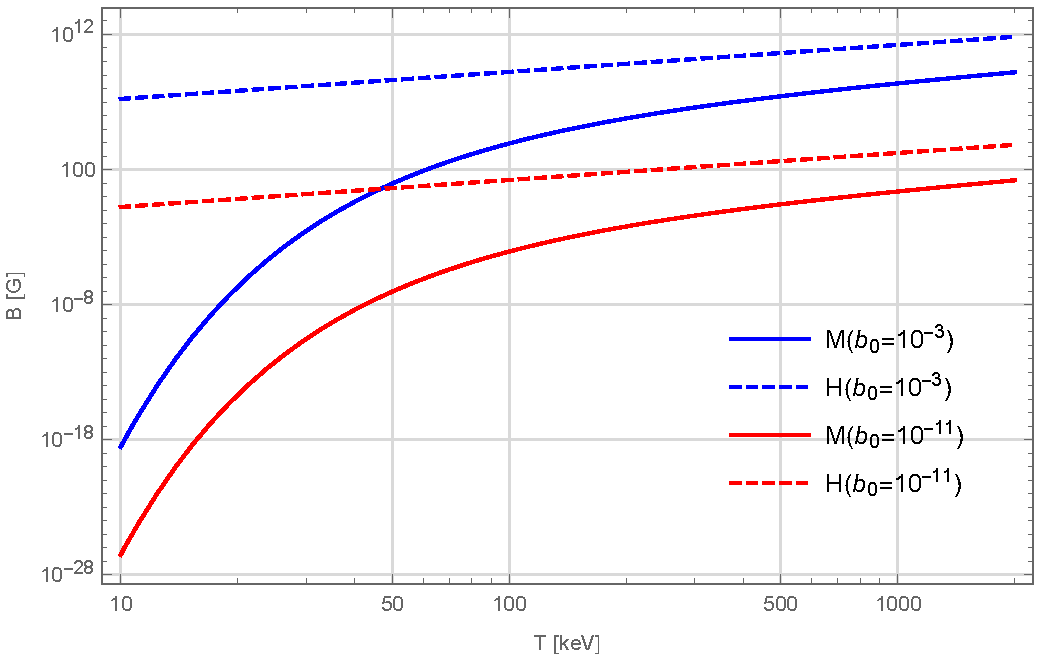
\includegraphics[width=\textwidth]{magplot.pdf}
    \caption{The dimensionless magnetization ${\cal M}/{\cal H}_{C}$ of the primordial $e^{+}e^{-}$ plasma is plotted as a function of temperature. The lower (solid red) and upper (solid blue) bounds for cosmic magnetic scale $b_{0}$ are included. The external magnetic field $B/H_{C}$ is also plotted in for lower (dashed red) and upper (dashed blue) bounds. The spin fugacity is set to unity $\xi=1$. {\xred Have this plot replaced with non-zero chemical potential. Caption is good.}}
    \label{magnetization} 
\end{figure}
%%%%%%%%%%%%%%%%%%%%%%%%%%%%%%%%%%%%%%%
\noindent The magnetization of the $e^{+}e^{-}$ plasma described by the partition function in \req{boltzmann} can be written as
\begin{align}
    \label{defmagetization}
    {\cal M}\equiv\frac{T}{V}\frac{\partial}{\partial{\cal B}}\ln{{\cal Z}_{e^{+}e^{-}}} = \frac{T}{V}\left(\frac{\partial b_{0}}{\partial{\cal B}}\right)\frac{\partial}{\partial b_{0}}\ln{{\cal Z}_{e^{+}e^{-}}}\,,\qquad\frac{\partial b_{0}}{\partial{\cal B}}=\frac{q}{T^{2}}\,.
\end{align}
Magnetization arising from other components in the cosmic gas (protons, neutrinos, etc...) could in principle also be included. In the context of MHD, primordial magnetogenesis from neutrino interactions in the electron-positron epoch was considered in~\cite{perrone2021neutrinoelectron}. We also introduce dimensionless units for magnetization by defining the critical displacement field
\begin{align}
    {\cal H}_{C}\equiv\frac{m_{e}^{2}}{q}\,.
\end{align}
The total magnetization ${\cal M}$ can be broken into the sum of spin parallel ${\cal M}_{+}$ and spin anti-parallel ${\cal M}_{-}$ magnetization. We note that the expression for the magnetization simplifies significantly for $g=2$ which is the \lq\lq cusp\rq\rq\ gyro-magnetic factor~\cite{rafelski2022study} of the Dirac particle. For illustration, the $g=2$ magnetization from \req{defmagetization} is then
\begin{align}
    \label{g2magplus}
    \frac{{\cal M}_{+}}{{\cal H}_{C}}&=\frac{q^{2}}{2\pi^{2}}\frac{T^{2}}{m_{e}^{2}}\xi^{-1}\cosh{\frac{\mu}{T}}\left[\frac{1}{2}x_{+}K_{1}(x_{+})+\frac{b_{0}}{6}K_{0}(x_{+})\right]\,,\qquad x_{+}=\left(\frac{m_{e}}{T}\right)\,,\\
    \label{g2magminus}
    \frac{{\cal M}_{-}}{{\cal H}_{C}}&=-\frac{q^{2}}{2\pi^{2}}\frac{T^{2}}{m_{e}^{2}}\xi\cosh{\frac{\mu}{T}}\left[\left(\frac{1}{2}+\frac{b_{0}^{2}}{12x_{-}^{2}}\right)x_{-}K_{1}(x_{-})+\frac{b_{0}}{3}K_{0}(x_{-})\right]\,,\qquad x_{-}=\sqrt{\frac{m_{e}^{2}}{T^{2}}+2b_{0}}\,.
\end{align}
The expressions in \req{g2magplus} and \req{g2magminus} are only modified by a small amount by the present of anomalous magnetic moment as the $g$-factor of the electron is only slightly above two at $g\simeq2.00232$~\cite{tiesinga2021codata}.
 
Of interest is the determination of the magnetization per particle

%%%%%%%%%%%%%%%%%%%%%%%%%%%%%%%%%%%%%%%
\section{Closing}
\label{sec:conclusions}
\noindent tbw
\section{Snippets to Place}
While the universe is nearly homogeneous and isotropic (the Cosmological Principle) on the largest scales, the inhomogeneities of matter (and dark matter) evolution are non-trivial and must generally be solved numerically using magneto-hydrodynamics (MHD)~\cite{melrose2008quantum,vazza2017simulations}.

%%%%%%%%%%%%%%%%%%%%%%%%%%%%%%%%%%%%%%%
\bibliographystyle{unsrtnat}
\bibliography{refs-plasma-partition}
%%%%%%%%%%%%%%%%%%%%%%%%%%%%%%%%%%%%%%%

\end{document}
